\documentclass{standalone}
\usepackage{tikz, xcolor}
\usetikzlibrary{shapes,arrows}

\begin{document}

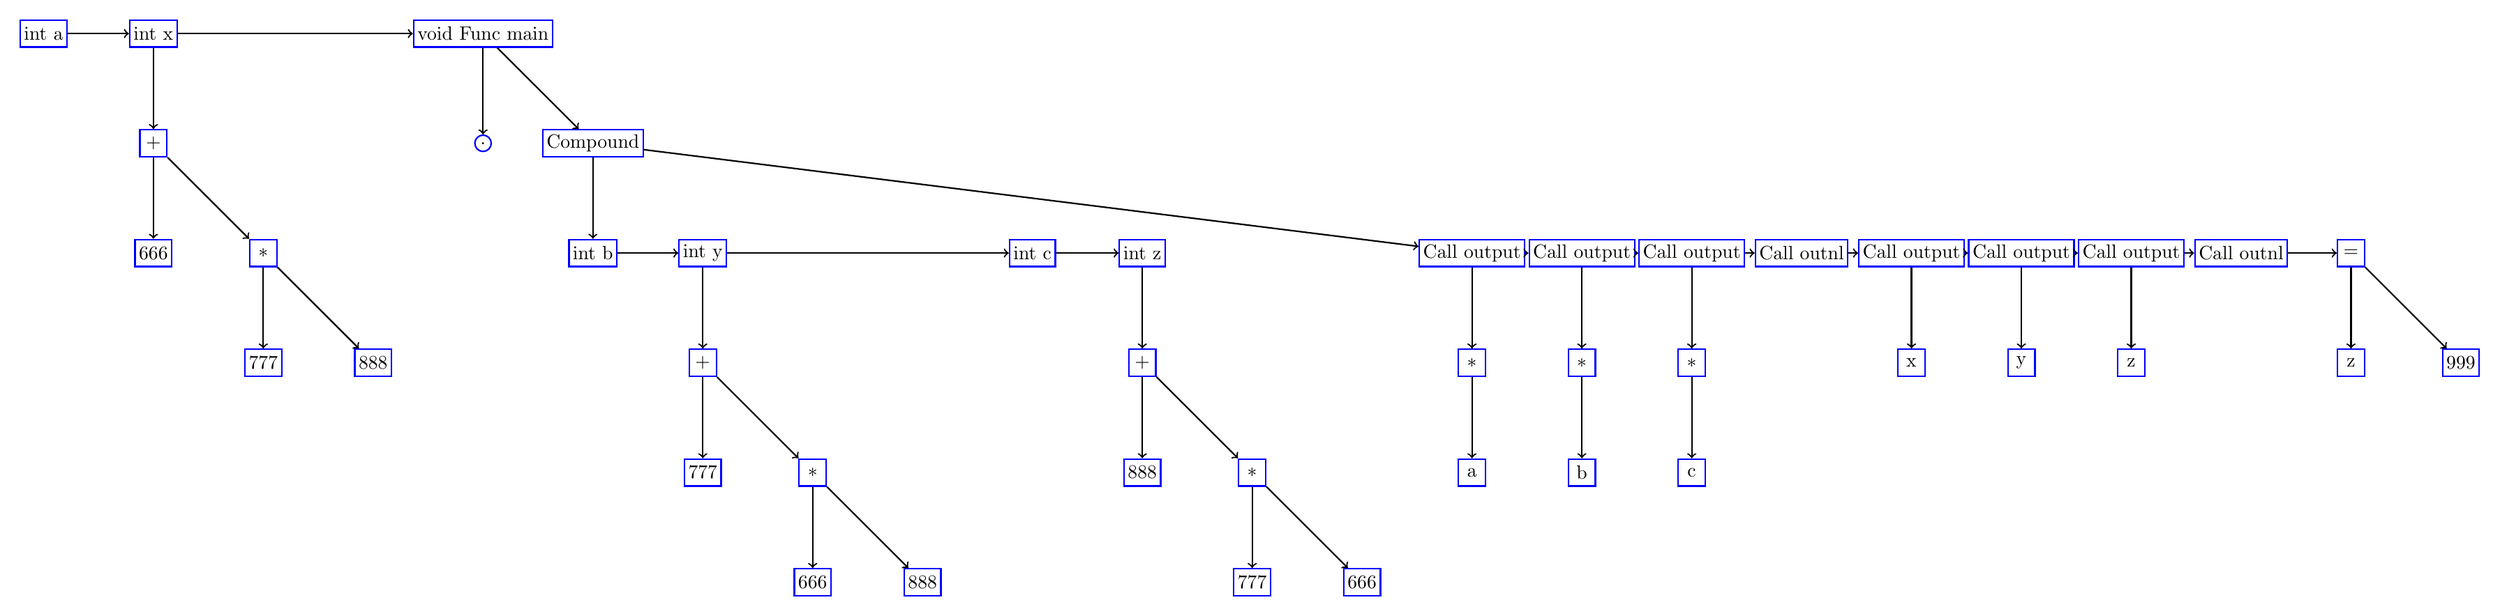
\begin{tikzpicture}[thick, scale=2.0]
\tikzstyle{vertexr}=[rectangle, draw=blue, thick, minimum size=14pt, inner sep=2pt]
\tikzstyle{vertexc}=[circle, draw=blue, thick, inner sep=2pt]
\tikzstyle{drawstyle}=[thick, ->]

\node[vertexr] (G0x0) at (0,0) {int a};
\node[vertexr] (G1x0) at (1,0) {int x};
\node[vertexr] (G1x1) at (1,-1) {$+$};
\node[vertexr] (G1x2) at (1,-2) {666};
\draw[drawstyle] (G1x1) -- (G1x2);
\node[vertexr] (G2x2) at (2,-2) {$*$};
\node[vertexr] (G2x3) at (2,-3) {777};
\draw[drawstyle] (G2x2) -- (G2x3);
\node[vertexr] (G3x3) at (3,-3) {888};
\draw[drawstyle] (G2x2) -- (G3x3);
\draw[drawstyle] (G1x1) -- (G2x2);
\draw[drawstyle] (G1x0) -- (G1x1);
\node[vertexr] (G4x0) at (4,0) {void Func main};
\node[vertexc] (G4x1) at (4,-1) {.};
\draw[drawstyle] (G4x0) -- (G4x1);
\node[vertexr] (G5x1) at (5,-1) {Compound};
\node[vertexr] (G5x2) at (5,-2) {int b};
\node[vertexr] (G6x2) at (6,-2) {int y};
\node[vertexr] (G6x3) at (6,-3) {$+$};
\node[vertexr] (G6x4) at (6,-4) {777};
\draw[drawstyle] (G6x3) -- (G6x4);
\node[vertexr] (G7x4) at (7,-4) {$*$};
\node[vertexr] (G7x5) at (7,-5) {666};
\draw[drawstyle] (G7x4) -- (G7x5);
\node[vertexr] (G8x5) at (8,-5) {888};
\draw[drawstyle] (G7x4) -- (G8x5);
\draw[drawstyle] (G6x3) -- (G7x4);
\draw[drawstyle] (G6x2) -- (G6x3);
\node[vertexr] (G9x2) at (9,-2) {int c};
\node[vertexr] (G10x2) at (10,-2) {int z};
\node[vertexr] (G10x3) at (10,-3) {$+$};
\node[vertexr] (G10x4) at (10,-4) {888};
\draw[drawstyle] (G10x3) -- (G10x4);
\node[vertexr] (G11x4) at (11,-4) {$*$};
\node[vertexr] (G11x5) at (11,-5) {777};
\draw[drawstyle] (G11x4) -- (G11x5);
\node[vertexr] (G12x5) at (12,-5) {666};
\draw[drawstyle] (G11x4) -- (G12x5);
\draw[drawstyle] (G10x3) -- (G11x4);
\draw[drawstyle] (G10x2) -- (G10x3);
\draw[drawstyle] (G9x2) -- (G10x2);
\draw[drawstyle] (G6x2) -- (G9x2);
\draw[drawstyle] (G5x2) -- (G6x2);
\draw[drawstyle] (G5x1) -- (G5x2);
\node[vertexr] (G13x2) at (13,-2) {Call output};
\node[vertexr] (G13x3) at (13,-3) {$*$};
\node[vertexr] (G13x4) at (13,-4) {a};
\draw[drawstyle] (G13x3) -- (G13x4);
\draw[drawstyle] (G13x2) -- (G13x3);
\node[vertexr] (G14x2) at (14,-2) {Call output};
\node[vertexr] (G14x3) at (14,-3) {$*$};
\node[vertexr] (G14x4) at (14,-4) {b};
\draw[drawstyle] (G14x3) -- (G14x4);
\draw[drawstyle] (G14x2) -- (G14x3);
\node[vertexr] (G15x2) at (15,-2) {Call output};
\node[vertexr] (G15x3) at (15,-3) {$*$};
\node[vertexr] (G15x4) at (15,-4) {c};
\draw[drawstyle] (G15x3) -- (G15x4);
\draw[drawstyle] (G15x2) -- (G15x3);
\node[vertexr] (G16x2) at (16,-2) {Call outnl};
\node[vertexr] (G17x2) at (17,-2) {Call output};
\node[vertexr] (G17x3) at (17,-3) {x};
\draw[drawstyle] (G17x2) -- (G17x3);
\node[vertexr] (G18x2) at (18,-2) {Call output};
\node[vertexr] (G18x3) at (18,-3) {y};
\draw[drawstyle] (G18x2) -- (G18x3);
\node[vertexr] (G19x2) at (19,-2) {Call output};
\node[vertexr] (G19x3) at (19,-3) {z};
\draw[drawstyle] (G19x2) -- (G19x3);
\node[vertexr] (G20x2) at (20,-2) {Call outnl};
\node[vertexr] (G21x2) at (21,-2) {=};
\node[vertexr] (G21x3) at (21,-3) {z};
\draw[drawstyle] (G21x2) -- (G21x3);
\node[vertexr] (G22x3) at (22,-3) {999};
\draw[drawstyle] (G21x2) -- (G22x3);
\draw[drawstyle] (G20x2) -- (G21x2);
\draw[drawstyle] (G19x2) -- (G20x2);
\draw[drawstyle] (G18x2) -- (G19x2);
\draw[drawstyle] (G17x2) -- (G18x2);
\draw[drawstyle] (G16x2) -- (G17x2);
\draw[drawstyle] (G15x2) -- (G16x2);
\draw[drawstyle] (G14x2) -- (G15x2);
\draw[drawstyle] (G13x2) -- (G14x2);
\draw[drawstyle] (G5x1) -- (G13x2);
\draw[drawstyle] (G4x0) -- (G5x1);
\draw[drawstyle] (G1x0) -- (G4x0);
\draw[drawstyle] (G0x0) -- (G1x0);
\end{tikzpicture}
\end{document}
Number of warnings: 0
Number of errors: 0
